\chapter{Advanced Tie Points}

%=======================================================================================================
\section{Changing default detector in {\tt  XML\_User/}}


There exist different implemantation of Sift detector and Ann matchor in MicMac. The newest one offer
more option, while the oldest have been more tested \dots 

To change the default behaviour you must edit your {\tt MM-Environment.xml} in the folder {\tt include/XML\_User/}.
For example :



\begin{verbatim}
<MMUserEnvironment>
    <TiePDetect> mm3d:Digeo </TiePDetect>
    <TiePMatch > mm3d:Ann </TiePMatch>
</MMUserEnvironment>
\end{verbatim}

Note that the {\tt mm3d:Digeo} implementation of SIFT detector offers several advantages :

\begin{enumerate}
   \item faster, specially in the gaussian computation;

   \item you can use the {\tt NoMax} and {\tt NoMin} options in {\tt Tapioca}, to supress the Min (or Max) in sift detection.
         This divides by $2$ the number of tie points, while conserving the same
         multiple tie point ratio (as at $99.99\dots \%$ a max is never a good homolog of a min).
\end{enumerate}

The default tie point detector is {\tt mm3d:Sift}.


%=======================================================================================================
\section{Filtering tie points in {\tt HomolFilterMasq}}


This command can be used when you have the necessary spatial information to retrieve false
tie points.

The command {\tt HomolFilterMasq} can do some filtering on tie points. The masking
process can be purerly in image geometry or can be done in some ground geometry.

\begin{verbatim}
 mm3d HomolFilterMasq
*****************************
*  Help for Elise Arg main  *
*****************************
Mandatory unnamed args : 
  * string :: {Full name (Dir+Pat)}
Named args : 
  * [Name=PostPlan] string :: {Post to plan, Def : toto ->toto_Masq.tif like with SaisieMasq}
  * [Name=GlobalMasq] string :: {Global Masq to add to all image}
  * [Name=KeyCalculMasq] string :: {For tuning masq per image}
  * [Name=KeyEquivNoMasq] string :: {When given if KENM(i1)==KENM(i2), don't masq}
  * [Name=Resol] REAL :: {Sub Resolution for masq storing, Def=10}
  * [Name=ANM] bool :: {Accept no mask, def = true if MasqGlob and false else}
  * [Name=ExpTxt] bool :: {Ascii format for in and out, def=false}
  * [Name=PostIn] string :: {Post for Input dir Hom, Def=}
  * [Name=PostOut] string :: {Post for Output dir Hom, Def=MasqFiltered}
  * [Name=OriMasq3D] string :: {Orientation for Masq 3D}
  * [Name=Masq3D] string :: {File of Masq3D, Def=AperiCloud_${OriMasq3D}.ply}
  * [Name=SelecTer] Pt2dr :: {[Per,Prop] Period of tiling on ground selection, Prop=proporion of selected}
  * [Name=DistId] REAL :: {Supress pair such that d(P1,P2) < DistId, def unused}
\end{verbatim}

The main option are :

\begin{enumerate}
    \item {\tt PostPlan} for example set {\tt PostPlan=titi} if there is masq per image and for each image 
          {\tt Image.tif} the masq if {\tt Image\_Masqtiti.tif}, by default will generate an error if this
          image does not exist, set {\tt ANM=true} if you know that non existing images are normal;

    \item {\tt GlobalMasq} if masq common to all images exist (for example with fiducial marqs);

    \item {\tt KeyCalculMasq} , sometime you may have many images and a few masq, each masq being applyable
          for a group of images; use this option with much be a computation key desrcibed in
          {\tt MicMac-LocalChantierDescripteur.xml}

    \item {\tt Masq3D} , a file for 3D masq as seized by {\tt SaisieMasqQT}, the orientation {\tt OriMasq3D} 
          must be initialized;

    \item {\tt SelecTer} , can be used to decrease the number of tie points while maintaining the proportion
          of multiplicity;  if {\tt SelecTer=[Per,Prop]}, then in each tile of size $S=Per*Resol$  in the ground coordinate
          \footnote{$Resol$ being the average ground resolution} the point are selected in the subtile of 
          size $S * \sqrt{Prop}$
    
    \item {\tt DistId} supress the pair of point $P_1,P_2$ such that $d(P_1,P_2)<DistId$, for example,
          this can be usefull when the acquistion was made using a turn table to automatically supress the
          point on the background;
    
\end{enumerate}



%=======================================================================================================

\section{Merging Tie point from multiple view with {\tt HomolMergePDVUnik}}

This command correspond to rather special case, when you have a set of camera that do not move (or form a rigid block) and the scene is moving.
For example :

\begin{itemize}
    \item there is three fixed camera $A,B,C$;
    \item at time $1,2,3,4$ someone is moving in fornt of the camera and the images $A_1,A_2, \dots C_3,C_4$ were acquired ;
\end{itemize}

It is not possible to make some standard photogrammetric processing on $A_1,A_2, \dots C_3,C_4$ as the scene is not static.
By the way if we knew the pose  $P_A,P_B,P_C$ of the camera, then  all the homologous points $(A_1,B_1), (A_2,B_2) \dots (A_4,B_4)$ 
would be compatible witj $P_A$ and $P_B$, which means that we can merge this tie points in a unique file that can be used
to estimate $P_A$ and $P_B$; and the same with $A,C$ and $B,C$. 


The command  {\tt HomolMergePDVUnik} does this merging, in fact you can consider that the tie-points 
obtained are more or less resulting are some kind of merging from the different scene. 

\begin{verbatim}
mm3d HomolMergePDVUnik
*****************************
*  Help for Elise Arg main  *
*****************************
Mandatory unnamed args : 
  * string :: {Full name (Dir+Pat)}
  * string :: {Dir of external point}
Named args : 
  * [Name=PostIn] string :: {Post for Input dir Hom, Def=}
  * [Name=PostOut] string :: {Post for Output dir Hom, Def=MasqFusion}
  * [Name=ExpTxt] bool :: {Ascii format for in and out, def=false}
  * [Name=DirN] vector<std::string> :: {Supplementary dirs 2 merge}
\end{verbatim}



%=======================================================================================================
\section{Tie points on low contrast images usign {\tt SFS} in {\tt MicMac-LocalChantierDescripteur.xml}}


The current implementation of SIFT++ used in MicMac is not fully invariant to scaling/translation in radiometry. This may be a problem in case of acquisitions having a good SNR but with low contrast in the scene; in this case, thanks to good SNR there is potential information to get tie points, but as this information is assimilated to noise, it cannnot be extracted.

To overcome this problem, it is possible to require that MicMac computes some contrast enhancement on images before computing SIFT points. Although this method is not optimal (it would be better to modify the SIFT++ Kernel), it has the advantage of existing\dots



The figure~\ref{FIG:SF:Det} presents an image without enhancement, in its original form, and the same image after enhancement. The figure~\ref{FIG:SF:TieP} presents the detected tie points; we notice that the spatial density of tie points is much higher on enhanced image.

Of course, the enhanced images are fairly artificial, as it can be seen on figure~\ref{FIG:SF:Img} that presents a full image before and after enhancement. So if this option is activated, the enhanced images are used only for the tie points steps (which are developed as specific "hidden files" in folder {\tt Tmp-MM-Dir}).


To activate this option, the {\tt NKS-Assoc-SFS} must be changed in the {\tt MicMac-LocalChantierDescripteur.xml}. It must return {\tt SFS} instead of the default value {\tt NONE}. For example:

\begin{verbatim}
    <KeyedNamesAssociations>
        <Calcs>
            <Arrite>  1 1 </Arrite>
            <Direct>
                <PatternTransform> .* </PatternTransform>
                <CalcName>  SFS </CalcName>
            </Direct>
        </Calcs>
        <Key>   NKS-Assoc-SFS </Key>
    </KeyedNamesAssociations>
\end{verbatim}

\begin{figure}
\begin{center}
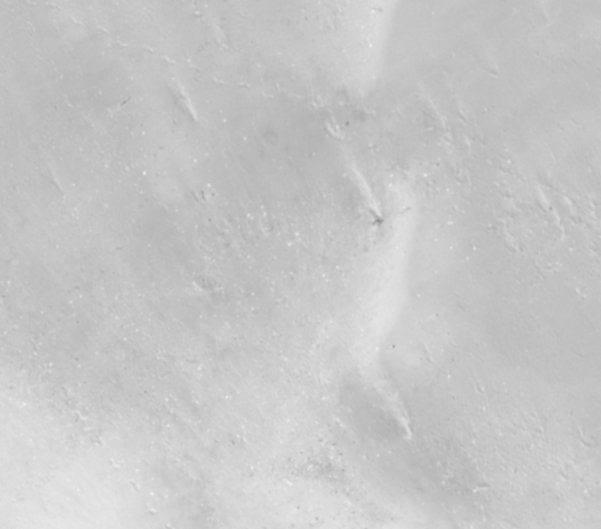
\includegraphics[width=0.4\textwidth]{FIGS/Tapioca-SFS/Detail-STD.jpg}
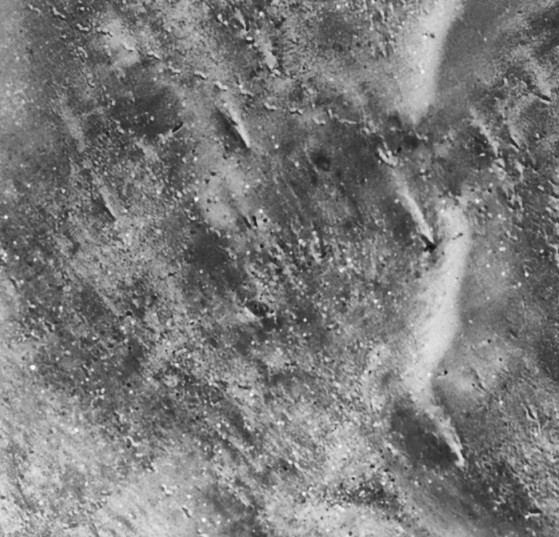
\includegraphics[width=0.4\textwidth]{FIGS/Tapioca-SFS/Detail-SFS.jpg}
\end{center}
\caption{Detail of image before and after enhancement}
\label{FIG:SF:Det}
\end{figure}


\begin{figure}
\begin{center}
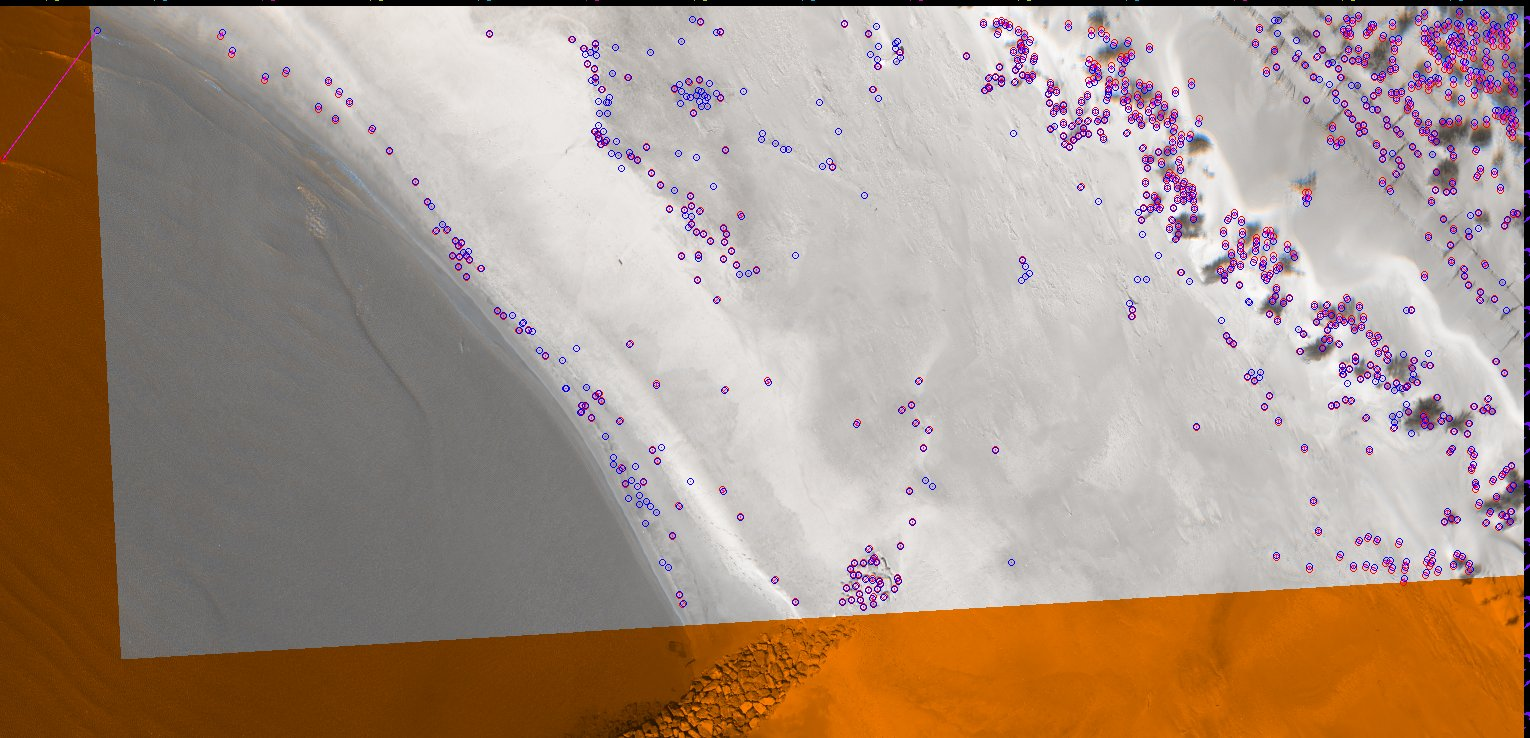
\includegraphics[width=0.95\textwidth]{FIGS/Tapioca-SFS/SIFT-STD.jpg}
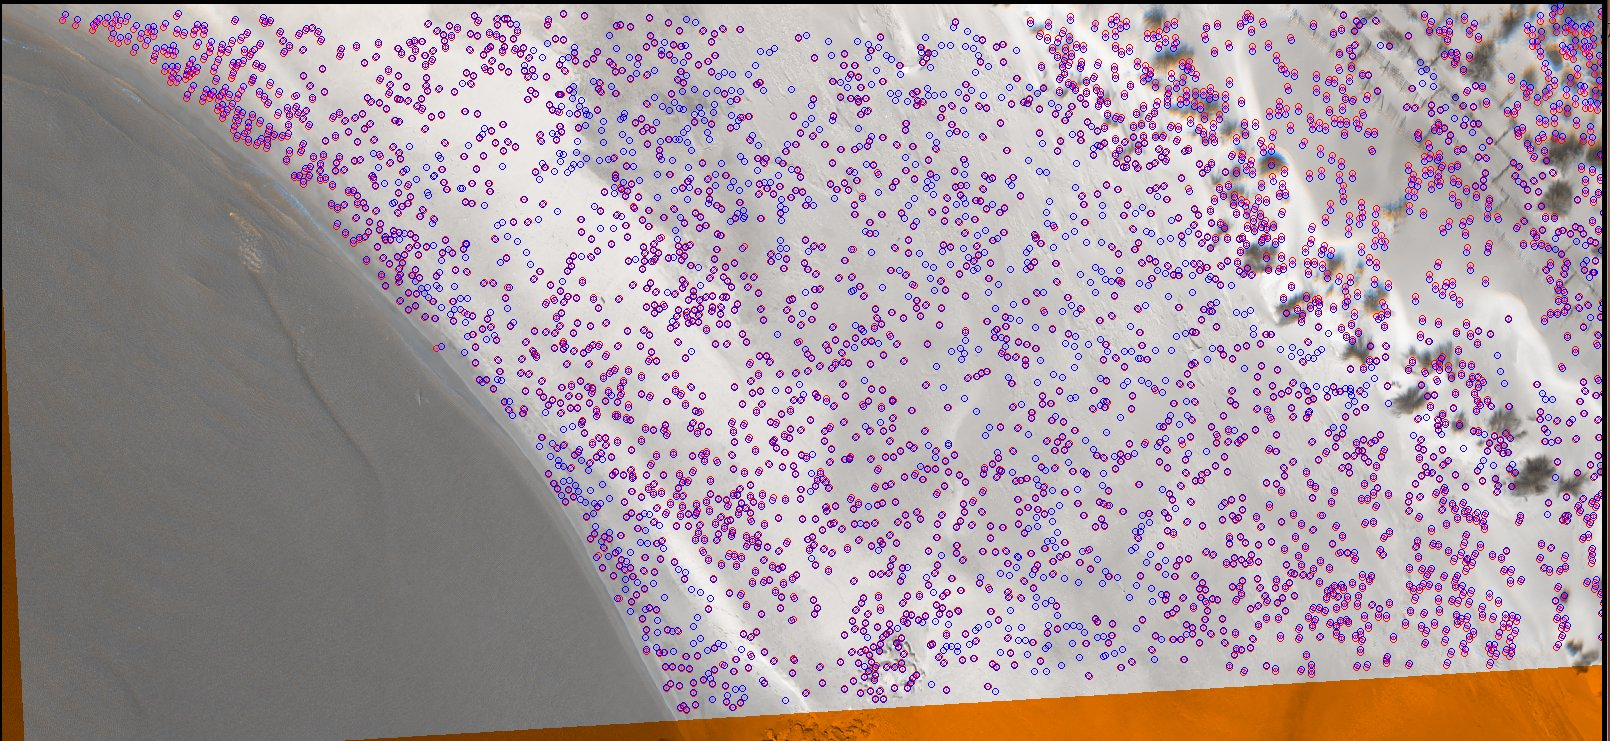
\includegraphics[width=0.95\textwidth]{FIGS/Tapioca-SFS/SIFT-SFS.jpg}
\end{center}
\caption{Tie points before and after enhancement}
\label{FIG:SF:TieP}
\end{figure}

\begin{figure}
\begin{center}
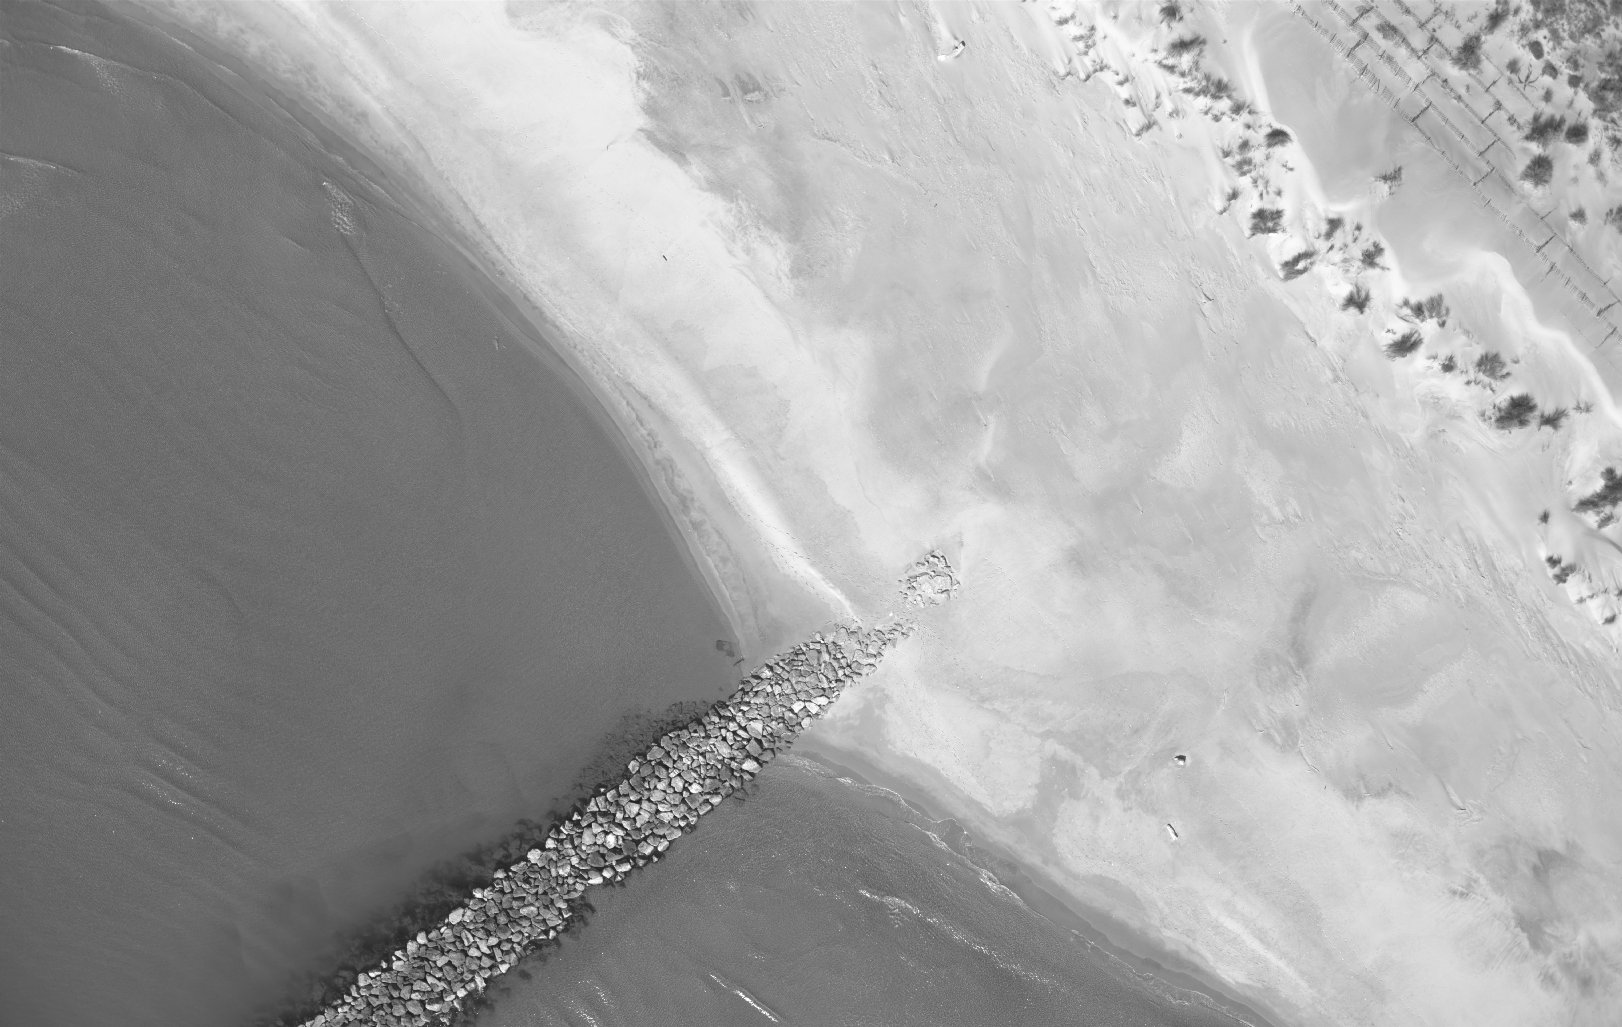
\includegraphics[width=0.95\textwidth]{FIGS/Tapioca-SFS/Im-STD.jpg}

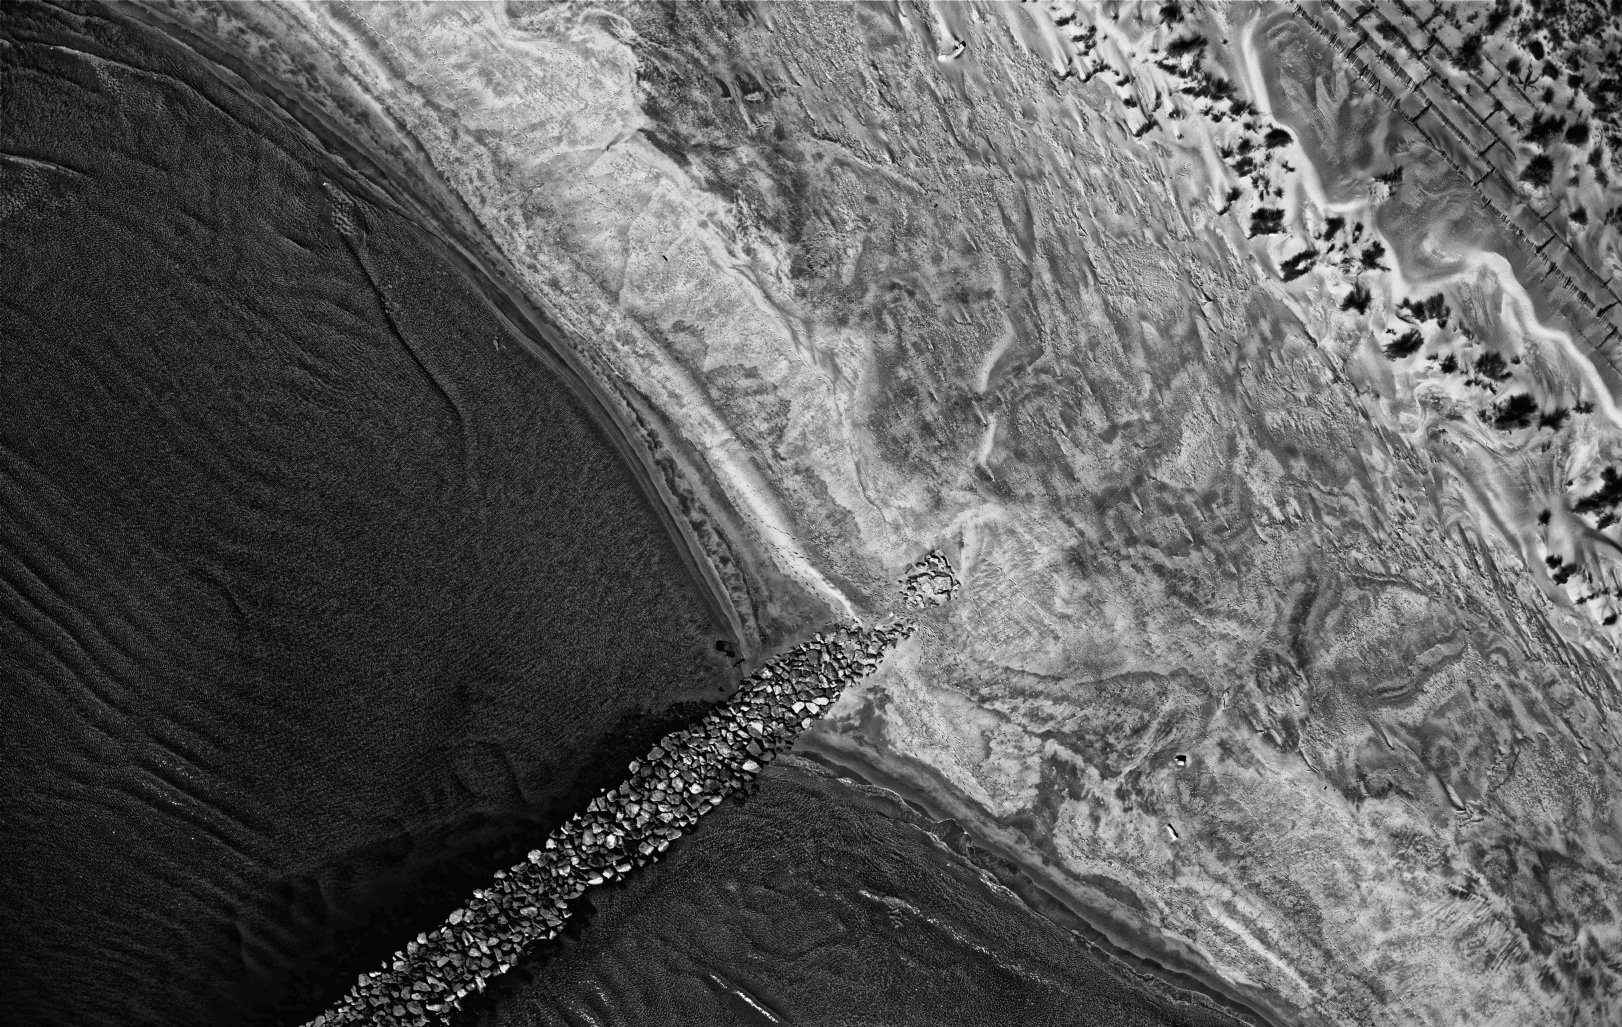
\includegraphics[width=0.95\textwidth]{FIGS/Tapioca-SFS/Im-SFS.jpg}
\end{center}
\caption{Global images before and after enhancement}
\label{FIG:SF:Img}
\end{figure}

%=======================================================================================================

\newpage

\subsection{Alternative syntax {\tt @SFS}}

It's also possible to use enhanced tie point, without {\tt MicMac-LocalChantierDescripteur.xml},
it suffice to add {\tt @SFS} at the {\tt Tapioca} command.

\section{Tie point reduction in {\tt RedTieP}}


This command can be used to reduce the number of tie points generated by \textit{Tapioca}. Currently it requires to format the \textit{Homol} folder into the Martini format, so before executing \textit{RedTieP} one has to execute the tool \textit{NO\_AllOri2Im} (obviously, after running \textit{Tapioca} to compute the tie-points):

The command {\tt RedTieP} keeps the tie-points that are present in a higher number of images and that guarantee a good distribution in the pixel-space of the images. 

\begin{verbatim}
 mm3d RedTieP
*****************************
*  Help for Elise Arg main  *
*****************************
Mandatory unnamed args : 
  * string :: {Pattern of images}
Named args : 
  * [Name=NumPointsX] INT :: {Target number of tie points between 2 images in x axis of 
                              image space, def=4}
  * [Name=NumPointsY] INT :: {Target number of tie points between 2 images in y axis of 
                              image space, def=4}
  * [Name=SubcommandIndex] INT :: {Internal use}
  * [Name=ExpSubCom] bool :: {Export the subcommands instead of executing them, def=false}
  * [Name=ExpTxt] bool :: {Export homol point in Ascii, def=false}
  * [Name=SortByNum] bool :: {Sort images by number of tie points, determining the order 
                              in which the subcommands are executed, def=0 
                              (sort by file name)}
  * [Name=Desc] bool :: {Use descending order in the sorting of images, def=0 (ascending)}
\end{verbatim}

The main options are :

\begin{enumerate}
\item The first option is mandatory and it is the patter to be used to select the images.

\item {\tt NumPointsX} and {\tt NumPointsY} represent the target number of tie-points between an image pair (specified as \textit{numY}, i.e. \textit{numPointsTarget=numX*numY}).
   
\item {\tt SortByNum} to select if the sorting by file name or by number of tie-points (default is to sort by file name). This sorting has effect on the order in the processing workflow, the first image in the sorted list is the first one that has its tie-points reduced.

\item {\tt Desc} to indicate if use ascending or descending order when sorting the images to decide (default is ascending).

\item {\tt ExpTxt} is a boolean indicating if reduced tie-point are dumped in binary or ASCII format (default is binary).

\item \textit{ExpSubCom} is used to export the commands to perform the tie-point reduction pipeline without actually executing it. This is used to execute the pipeline with an external parallelization tool (see section below)
\end{enumerate}


\subsection{Algorithm description}

\begin{itemize}
\item Select the images from the pattern defined by the user. 

\item Sort the images. By default by file name in ascending order (user can choose to sort by number of tie-points, and/or to use descending order). 

\item Execute a set of tasks, one for each image. Each task executes various steps:
   \begin{itemize}
   
   \item Define a master image, the image driving the tie-point reduction in this task.
   
   \item Find the related images. The related images are images that share tie-points with the master image. 
   
   \item Load the tie-points shared between the master image and each of the related images. If a related image was a master image in a earlier executed task the algorithm uses the list of tie-points produced in that task (instead of the original list of tie-points as provided by Tapioca).

   \item Perform the topological merging of tie-points into multi-tie-points. A multi-tie-point stores in how many images a related tie-point is present (multiplicity) and its positions in those images. 
   
   \item For all the images including the master and the related images: 
      \begin{itemize}
      \item Create a grid that divides the image pixel-space. 
      
      \item Fill in the grid with the loaded multi-tie-points.
      \end{itemize}      
      
   \item For each cell of the master image grid:
      \begin{itemize}
       \item Sort the multi-tie-points according to multiplicity.
       \item Attempt to remove all the multi-tie-points in the grid cell except the one with higher multiplicity. A multi-tie-point can be deleted if it meets the following conditions:
          \begin{itemize}
          \item Condition 1: It is not present in a related image that was master in an earlier executed task.
          \item For each related image where the multi-tie-point has a tie-point: (Condition 2) there is at least another tie-point in the current master grid cell that is also shared with the related image, and (Condition 3) there is at least another tie-point in the grid cell of the related image. 
          \end{itemize}
      \end{itemize}
   \item Store the tie-points which have not been marked as deleteable.
   \end{itemize}
\end{itemize}

\subsection{Parallelization}

The \textit{RedTieP} executes the sets of tasks that perform the tie-point reduction using a single process and in sequential order. However, these tasks could be parallelized if the parallelization schema guarantees that there are never two tasks accessing the same set of tie-points (i.e. accessing the same files). Each tasks has mutual exclusion with some other tasks. In order to parallelize them we use a workflow execution engine called Noodles (https://github.com/NLeSC/noodles). A script that uses Noodles can be found in \textit{scripts/noodles\_exe\_pararallel.py}.

In order to run \textit{RedTieP} and parallelize it with Noodles use:
\begin{verbatim}
 mm3d RedTieP  {Pattern of images} ExpSubCom=1 
 python {MicMac path}/scripts/noodles_exe_pararallel.py -j {num. threads} subcommands.json
\end{verbatim}

To install Noodles Python 3.5 is required. We recommend downloading and installing Anaconda (https://www.continuum.io/). Then set an environment with Python 3.5, activate it and download and install Noodles:
\begin{verbatim}
git clone https://github.com/NLeSC/noodles.git
cd noodles
git checkout devel
pip install .
\end{verbatim}

%=======================================================================================================

\section{Global and order-agnostic tie point reduction with {\tt Schnaps}}
The command {\tt Schnaps} is used to clean and reduce tie points before any orientation, and without needing any order in the pictures.
Its limitation is the user memory: it can't be used if computer RAM is lower than Homol directory size.

\begin{verbatim}
mm3d Schnaps
Schnaps : reduction of homologue points in image geometry
S trict           
C hoice of        
H omologous       
N eglecting       
A ccumulations on 
P articular       
S pots
*****************************
*  Help for Elise Arg main  *
*****************************
Mandatory unnamed args : 
  * string :: {Pattern of images}
Named args : 
  * [Name=HomolIn] string :: {Input Homol directory suffix (without "Homol")}
  * [Name=NbWin] INT :: {Minimal homol points in each picture (default: 1000)}
  * [Name=HomolOut] string :: {Output Homol directory suffix (default: _mini)}
  * [Name=ExpTxt] bool :: {Ascii format for in and out, def=false}
  * [Name=VeryStrict] bool :: {Be very strict with homols (remove any suspect), def=false}
  * [Name=PoubelleName] string :: {Where to write suspicious pictures names, def="Schnaps_poubelle.txt"}
\end{verbatim}

You can choose the Homol directory suffix for input and output. By default it uses ``Homol'' and creates a ``Homol\_mini'' directory for output.

The number of windows gives a clue about the number of tie points you will get.
You may get less points if there are no tie point in every window, and you may get more points if they have a great multiplicity.

The suspicious Homol points will be removed (then detecting bad loops of tie points), and the missing pairs will be completed (closing the loops).


\subsection{Algorithm}
{\tt Schnaps} computes a collection of Homol points, each recording its coordinates in every picture it appears.
When something is not coherent, the Homol point is discarded.

It then selects the best Homol point (multiplicity) in each sub-window of each picture.
When an Homol point is selected, it appears in every picture it is seen in.

The tie points packs are then created using every selected Homol and every combination of pictures.
This may create new links between pictures (mostly if you used {\tt Tapiocal Line} with a low number of adjacent image).

The {\tt VeryStrict} option makes {\tt Schnaps} check that every Homol has been seen in every couple Tapioca tested.


\subsection{Output}

\begin{figure}
\begin{center}
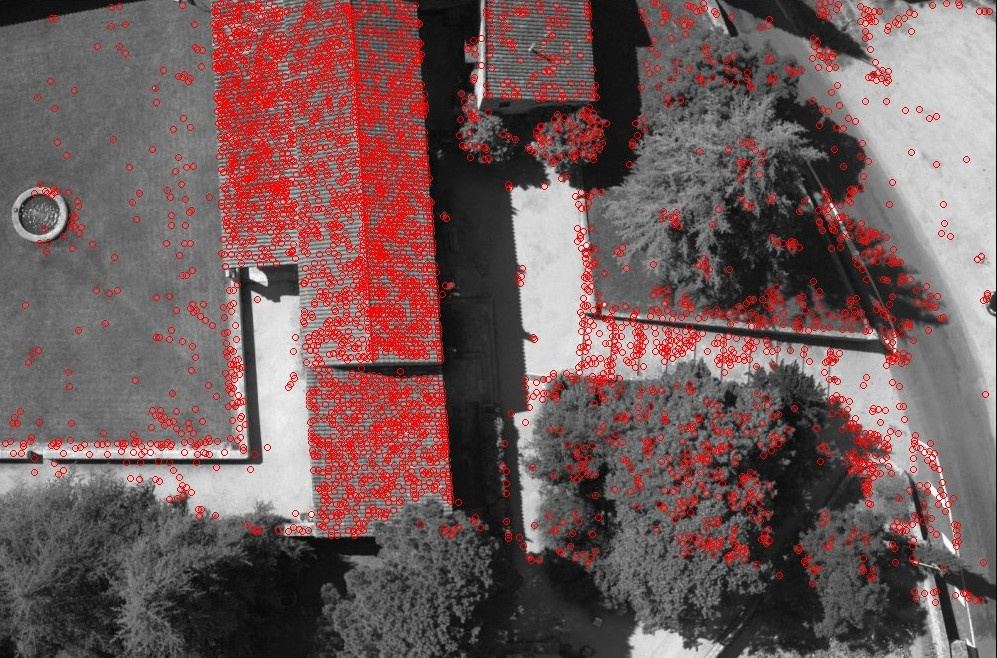
\includegraphics[width=0.49\textwidth]{FIGS/Schnaps/Schnaps_homol_all.jpg}
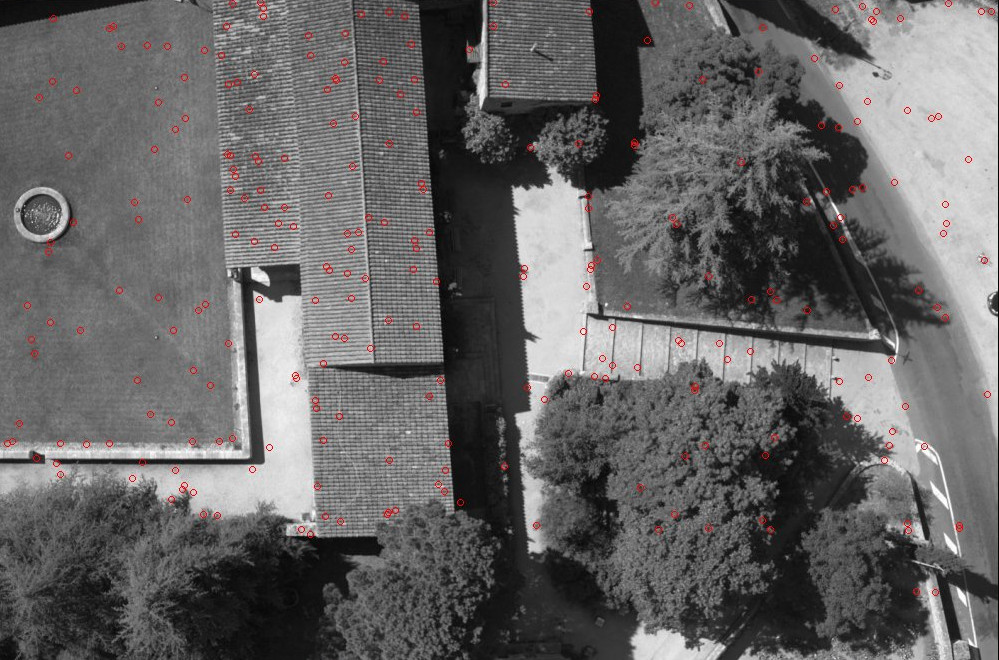
\includegraphics[width=0.49\textwidth]{FIGS/Schnaps/Schnaps_homol_100.jpg}
\end{center}
\caption{Tie points before and after Schanps with 100 sub-windows}
\end{figure}

{\tt Schnaps} will create a new directory with filtered tie points.
It will also evaluate the ``useful'' area of each picuture, and give a list of bad pictures (less than $25\%$ of the area used) in a file called {\tt Schnaps\_pictures\_poubelle.txt}. You may use it to clear your pictures list before Tapas.

Then computing orientations, filtered tie points may give bigger residuals since they are less redondant, but bascule tests show that the geometry is better
after filtering.

The orientation computation may also be faster if the number of points decreased, and {\tt Schnaps} also allows you to earn time with tighter {\tt Tapiocal Line},
since it will fill the links between pictures.

%=======================================================================================================
%=======================================================================================================
%=======================================================================================================

\section{Tie point reduction , with {\tt OriRedTieP} and {\tt Ratafia}}

\subsection{Generalities}

As the problem of tie points reduction has been very active, the command  {\tt OriRedTieP} 
and {\tt Ratafia} are alternative solution to  {\tt RedTieP} and {\tt Schnaps}; it is
expected that all these options correspond to complementary requirements and, as there is for 
now no deep comparison between them, the user is invited to test which one best comply with his particular problem.

For the two last one,  {\tt Ratafia} is a general command while {\tt OriRedTieP} is specialized for 
the quasi-vertical case (typically aerial or UAV) and it is expected to be a bit more
efficient in time and quality. Also, the difference between the two is tiny and it is more for historical reasons
that these two commands co-exist.



As with all tie-point reduction methods, the general  objective is to
limit the number of tie-point while maintening a good photogrammetric distribution. 
This rather general objective leads to the (somewhat contradictory) specifications :

\begin{itemize}
   \item select a minimal subset of tie points ;
   \item for each image, the subset of points where the image is present must have an homogoneous distribution
         (at least no hole, the notion of "hole" being controled by a threshold on distance);
   \item similarly, for each pair of images, the subset of points where the pair is present must have no hole;
   \item as far as possible, the point with high degree of multiplicity must be privileged (they give
         more "strength" to the photogrammetric canvas);

   \item if there is any means to evaluate the quality of tie points based on geometry, then privilege the points
         of good quality.

\end{itemize}

The algorithm for the two commands are pretty much the same. First we give a detailed description of {\tt OriRedTieP},
and after we describe  the few points that are  specific to {\tt Ratafia}.

% - - - - - - - - - - - - - - - - - - - - -- - - - - - -

\subsection{Tie point reduction , quasi-vertical case with {\tt OriRedTieP}}


      %   -    -    -    -    -    -

\subsubsection{Algorithm}

\label{TiePSel:GlobAlgo}

The command {\tt OriRedTieP} treats the problem of tie points reduction in the particular case
where the acquisition is quasi-vertical (generally applicable to UAV acquisition). 
It requires that a global orientation has been computed with the {\tt Martini}
command, as this orientation will be used both for computing the spatial distribution of
tie points and evaluate the quality of selected tie points (based on the reprojection precision).  As {\tt Martini} is memory efficient it can be executed
with almost arbitrary big data and there is no vicious circle.

To have a spatial distribution, for each tie point, the bundle intersection $P^{Gr}$ is computed
with the given orientation. The density of the tie point after reduction will be
controlled with a parameter $D_{Mul}$ which will be more or less the average
distance between $P^{Gr}$ of selected tie points. Also {\tt OriRedTieP} use only the $X,Y$
coordinate of $P^{Gr}$  and this is why it is only suited for quasi-vertical acquisition
\footnote{this may evolve later, but is due to the fact that now in the MicMac library there is quad-tree and no octree}


For its computation {\tt OriRedTieP} needs to evaluate the quality of each tie point, and it uses the
following formula :

\begin{equation}
   Qual= NbP * \frac{1}{1+(\frac{R}{R_m * Th_R})^2 } * (\frac{1}{2}+\frac{NbI}{NbI_0}) \label{QualTieP}
\end{equation}

Where :

\begin{itemize}
   \item $NbP$ is the number of pairs of images (for example for a point with multiplicity $4$,
         its value is between $3$ and $6$); this term privileges multiplicity of tie points;

   \item $R$ is the residual of reprojection and $R_m$ is the median of this residual on the data,
         $Th_R$ is a threshold (its default value is $2$); this term penalizes  high residual;

   \item $NbI$ is the number of images that are still uncovered (see bellow the definition, initialy no image is covered),
        and $NbI_0$ is the number of initial images; this term take into account the fact that once
        a tie point is partly covered, its potential contribution to the (photogrammetric) strength of the block decreases.

\end{itemize}

Finally, the tie points selection algoritm goes as follows :

\begin{itemize}
   \item extract the tie point $P$, not entirely covered, with the best quality (if none, end);
   \item add   $P$ to the set of selected tie points , then for all points $Q$ located within the distance of $D_{Mul}$ from the point $P$
         

   \begin{itemize}
         \item  for all images of $Q$, that are also in $P$, mark these images as covered;
         \item  if all images of $Q$ are covered, remove $Q$ ($Q$ is considered as no longer usefull if
                for each image  it contains, inside  a disc of ray $D_{Mul}$, there exists a selected tie point
                containing that image);
         \item  else, update the quality of  $Q$, according to formula~\ref{QualTieP} to take into account
                the fact that the number of uncovered images has decreased.
   \end{itemize}
\end{itemize}

This computation is done relatively fast, as a spatial indexe is used to extract the points in
a given disc, and a heap is used extract the tie points with highest quality. 

      %   -    -    -    -    -    -

\subsubsection{"Von Gruber" point}

The previous algorithm
guarantees that for each image, it has selected tie points with "no hole". But it does not
give the same waranty for a pair of images which may be a problem for the photogrammetric
strength of a bloc. The so named Von-Gruber \footnote{typically if the number of such points where $6$
their optimal distribution would be those of the Von-Gruber point in "classical" photogrammetry} 
points aim to fill
this gap. A second analys of the tie point is made , the algorithm being close
but slightly different from the previous one :


\begin{itemize}
   \item  all the pair  $I_1,I_2$ of images are considered  one after the other;

   \item  in the current step only tie point containing $I_1$ and $I_2$ are considered, let $S_{i1,i2}$ be this set;

   \item  let  $VG_{i1,i2}$ be the set  of tie point to be selected  for $I_1,I_2$;
          $VG_{i1,i2}$ is initialized with the points
          selected already in the previous steps and containing $I_1$ and $I_2$ 
          (i.e these point can come from global algorithm  in \ref{TiePSel:GlobAlgo}, or
          from  previous iteration, with other pairs, of these Von Gruber points).

\end{itemize}

Let :

\begin{equation}
 D^{VG}_{i1,i2}(Q)  = Min_{P \in VG_{i1,i2}} d(P,Q)
\end{equation}

We define the quality of potentiel point $Q$ by :


\begin{equation}
  Qual^{VG}(Q)  = \frac{D^{VG}_{i1,i2}(Q)}{1+2*\frac{R}{R_m}}
\end{equation}

This formula means that we want to add the tie points with the highest distance
from the already selected points (filling the "biggest hole") but also penalise points with high residual. The algorithm
is then :

\begin{itemize}
    \item let $D^{VG}_{max}$ be the max of $D^{VG}_{i1,i2}(Q)$ for $Q\in S_{i1,i2}$ ;
    \item let $D^{VG}_{Mul}$ be a threshold distance, by default $D^{VG}_{Mul} = 2 * D_{Mul}$
          (where $ D_{Mul}$ is the distance used for in \ref{TiePSel:GlobAlgo});

    \item while  $D^{VG}_{max} < D^{VG}_{Mul}$  add to  $VG_{i1,i2}$ the point maximizing $ Qual^{VG}$.
\end{itemize}

      %   -    -    -    -    -    -

\subsubsection{The command}

Before executing {\tt OriRedTieP}, {\tt Martini} must have been executed with the same option for the
calibration, for example :


\begin{verbatim}
mm3d Martini DSC01.*JPG
mm3d OriRedTieP DSC01.*JPG
\end{verbatim}

Or :

\begin{verbatim}
mm3d Martini DSC01.*JPG OriCalib=Ori-Calib/
mm3d OriRedTieP DSC01.*JPG OriCalib=Ori-Calib/
\end{verbatim}

As usual to know the parameters :


\begin{verbatim}
mm3d OriRedTieP -help
*****************************
*  Help for Elise Arg main  *
*****************************
Mandatory unnamed args : 
  * string :: {Pattern of images}
Named args : 
  * [Name=OriCalib] string :: {Calibration folder if any}
  * [Name=Prec2P] REAL :: {Threshold of precision for 2 Points}
  * [Name=KBox] INT :: {Internal use}
  * [Name=SzTile] INT :: {Size of Tiles in Pixel Def=2000}
  * [Name=DistPMul] REAL :: {Typical dist between pmult Def=200.000000}
  * [Name=MVG] REAL :: {Multiplier VonGruber}
  * [Name=Paral] bool :: {Do it paral, def=true}
  * [Name=VerifNM] bool :: {(Internal) Verification of Virtual Name Manager}
\end{verbatim}

The signification of the main parameters are :

\begin{itemize}
   \item mandatory parameter the pattern of images (must be a subset of the one used with {\tt Martini}).
   \item  {\tt OriCalib} must be coherent with the parameter name used in {\tt Martini};
   \item  {\tt DistPMul} controls the density of points per image and it's the average distance between the
          tie points; there is a waranty that for all images and the initial tie points, there exists
          a selected tie point at a distance inferior to  {\tt DistPMul}
   \item  {\tt MVG} controls the density of points per pair; for a given pair $I_1,I_2$ and 
          {\tt DistPMul}, the images will have a given density, but it does not give any guarantee of "goodness"
          on the points belonging to $I_1,I_2$, which may be a problem for the robustness;
          let $D'=MVG*DistPMul$, for each pair $I_1,I_2$   there is a guarantee 
          that for each tie points of $I_1,I_2$ , there exists
          a selected tie point of $I_1,I_2$ at a distance inferioir to  $D'$;
\end{itemize}


      %   -    -    -    -    -    -

\subsubsection{Memory issue and parallelization}


As the aim of {\tt OriRedTieP} is to be able to process big data set with standard memory,
obviously the tie points cannot be all loaded simultaneously. As ground coordinate can be
computed, it is easy to separate the problem in small tiles which are computed independantly
and this is what is done.

Also, one benefit of this tiling is that the tiles being independant, the computation can
be done in parallel and this is what is done.


% - - - - - - - - - - - - - - - - - - - - -- - - - - - -

\subsection{Tie point reduction , general case with {\tt Ratafia}}

\subsubsection{The algoritm}

The tool {\tt Ratafia} can deal with any kind of acquisition. The main difference with
{\tt OriRedTieP} is that the spatial indexation (computation of distance) is done in image geometry.
This has the following consequences :

\begin{itemize}
   \item the current computation  is done with a "master" image $I_0$;

   \item in this current computation  only the tie points that contains $I_0$ are considered;

   \item the position of a tie-point, used for distance computation, is the value of the point in $I_0$;

   \item to assure a complete coverage of the acquisition, each image at a certain point  will have to be the "master" image;

   \item as soon as the first image is processed,  some tie points are selected, and it must have an influence on 
         the computation of next images (as some points are already "covered" by the already selected tie points);

   \item so basically, the programm cannot be parallelized naively, as the result of each selected master
         image may influence the selection on remaining images;

   \item however when two images $I_1$ and $I_2$ have no common points, there is no contradiction to execute the computation
         in parallel  (their tie points are completely separated; remember : for example when computing $I_1$ only the points 
         containing $I_1$ are considered).
\end{itemize}

The algorithm used by  {\tt Ratafia}  is the following ;

\begin{itemize}
   \item create a partition of the images $P=\{S_1,S_2,...S_N\}$ such that
         $\forall i,j,n$  with $I_i \in S_n$ and $I_j \in S_n$ we have $ TieP(I_i,I_j) = \emptyset $; 
         in fact this condition is not fixed strictly, and it is accepted that the
          number of tie points may be equal to a very few percentage of the points;
 
   \item sequentially process each element of the partition $S_1, S_2 \dots $, for each element $S_k$  do:

   \begin{itemize}
        \item let  $S_k =\{I_1, I_2 , \dots \} $, for each element $I_k$  do in parallel :
        \begin{itemize}
              \item read the already computed tie points, and add them to initially selected tie points;
              \item consider only multiple tie points linked to $I_k$, and use $I_k$ coordinates for
                    indexation;
              \item then do the same computation as  in  \ref{TiePSel:GlobAlgo} , 
              \item save only the tie points that were added at this step.
        \end{itemize}
   \end{itemize}
\end{itemize}


There is also a slight difference with {\tt OriRedTieP}, as there is no need for a global $3d$ geometry. Moreover, as the tool {\tt Martini} (that otherwise furnises the global geometry) is still in progress, the evaluation of the residual is
not made on a global orientation, but on the relative orientation between the pair of images. This is
theoretically not as good, because intersection of all images $2$ by $2$ is not equivalent to a global
intersection, but the difference is tiny. Nonetheless, when {\tt Martini} will be completely finished, there
will be an option to use the $3d$ geometry.


\subsubsection{The command line}

Before executing {\tt Ratafia}, compute the relative orientation between pairs of images with
the  command {\tt TestLib NO\_AllOri2Im}
(first step of {\tt Martini}). Remember to execute the command with the same calibration option, for example :


\begin{verbatim}
mm3d TestLib NO_AllOri2Im DSC01.*JPG
mm3d Ratafia DSC01.*JPG
\end{verbatim}

Or :

\begin{verbatim}
mm3d TestLib NO_AllOri2Im DSC01.*JPG OriCalib=Ori-Calib/
mm3d Ratafia DSC01.*JPG OriCalib=Ori-Calib/
\end{verbatim}


Also, runing {\tt Martini} instead of  {\tt TestLib NO\_AllOri2Im} would have worked perfectly, 
but the global orientation would not have been used. As usual to know the parameters :

\begin{verbatim}
mm3d Ratafia -help
*****************************
*  Help for Elise Arg main  *
*****************************
Mandatory unnamed args : 
  * string :: {Pattern of images}
Named args : 
  * [Name=OriCalib] string :: {Calibration folder if any}
  * [Name=LevelOR] INT :: {Level Or, 0=None,1=Pair,2=Glob, (Def=1)}
  * [Name=NbP] INT :: {Nb Process, def use all}
  * [Name=RecMax] REAL :: {Max overlap acceptable in two parallely processed images}
  * [Name=ShowP] bool :: {Show Partition (def=false)}
  * [Name=SzPixDec] REAL :: {Sz of decoupe in pixel}
  * [Name=TEO] bool :: {Test Execution OriRedTieP ()}
  * [Name=Out] string :: {Folder dest => Def=-Ratafia}
  * [Name=DistPMul] REAL :: {Average dist}
  * [Name=MVG] REAL :: {Multiplier VonGruber, Def=2.000000}
  * [Name=Paral] bool :: {Do it in parallel}
  * [Name=DCA] bool :: {Do Complete Arc (Def=false)}
  * [Name=UseP] bool :: {Use prec to avoid redundancy (Def=true), tuning only}
\end{verbatim}

The meaning of main parameters is:

\begin{itemize}
   \item mandatory parameter the pattern of images (must be a subset of the one used with {\tt TestLib NO\_AllOri2Im}).

   \item  {\tt OriCalib} must be coherent with the parameter of same name used in {\tt TestLib NO\_AllOri2Im};

   \item  {\tt NbP} number of processes on which the parallelization is done:

   \item  {\tt RecMax} proportion of common tie point where images are considered deconnected (def=$\frac{1}{100}$);

   \item  {\tt DistPMul} average distance in pixel between tie points;

   \item  {\tt DCA} Do Complete Arc, if this option is active an attempt will be made to complete the incomplete
          tie points; for example, with a triple tie point comming from the fusion of $(I_1,p_1,I_2,p_2)$ and
          $(I_2,p_2,I_3,p_3)$; during the export, the $(I_1,p_1,I_3,p_3)$ will be added (i) if not already present, and if (ii)
          the geometric quality is sufficient (based on relative orientation); default value is false as it 
          seems not to improve any accuracy;
\end{itemize}


{\tt Ratafia} output some messages :

\begin{verbatim}
mm3d Ratafia DSC01.*JPG OriCalib=Ori-Calib/
=======    Done 0  Part on 8 ================
=======    Done 1  Part on 8 ================
=======    Done 2  Part on 8 ================
=======    Done 3  Part on 8 ================
=======    Done 4  Part on 8 ================
=======    Done 5  Part on 8 ================
=======    Done 6  Part on 8 ================
=======    Done 7  Part on 8 ================
----------------------------- NbP=1246 --------------------
 For muliplicity 2 %=28.3307 N=353 D=1
 For muliplicity 3 %=25.1204 N=313 D=2.59425
 For muliplicity 4 %=15.7303 N=196 D=4.62245
 For muliplicity 5 %=10.7544 N=134 D=7.36567
 For muliplicity 6 %=9.55056 N=119 D=10.6975
 For muliplicity 7 %=5.939 N=74 D=14.5676
 For muliplicity 8 %=3.29053 N=41 D=17.7805
 For muliplicity 9 %=1.28411 N=16 D=20.875
 ***************************************************
 *                                                 *
 *       R-eduction                                *
 *       A-utomatic of                             *
 *       T-ie points                               *
 *       A-iming to get                            *
 *       F-aster                                   *
 *       I-mage                                    *
 *       A-erotriangulation                        *
 *                                                 *
 ***************************************************
\end{verbatim}

The first series of message is just an indication of the computation. The second
series is some statistic on the distribution of tie points  :

\begin{itemize}
   \item let me comment {\tt For muliplicity 3 \%=25.1204 N=313 D=2.59425} :
   \begin{itemize}
   \item there is $313$ point of multiplicity $3$, they represent $25.1\%$ the average
         of number of couple is $2.59$ (the value being theorically between $2$ and $3$).
   \end{itemize}
   
\end{itemize}


%=======================================================================================================

\section{New Tie Points format}


% - - - - - - - - - - - - - - - - - - - - - - - - - - -
\subsection{Motivation}

The original tie points format, is made of independant file for each pair of images.
The multiple tie point are constructed "on the fly" when needed.  If this format 
is very flexible, it has also some drawback in efficiency. The main requirement of
the new format for future optimisation in MicMac is :

\begin{itemize}
   \item  explicit representation of multiple tie points;
   \item  gather at the same location the points that correspond at the same subset of images.
\end{itemize}


% - - - - - - - - - - - - - - - - - - - - - - - - - - -
\subsection{Format specification}


\subsubsection{Text format}

Here is an extract of a file in text mode :


{\tiny
\begin{verbatim}
BeginHeader-MicMacTiePointFormat
   Version=0.0.0
EndHeader
#=*=*=*=*=*=*=*=*=*=*=*=*=*=*=*=*=
15 #Nb Images
IMGP7040.JPG=0
....
IMGP7054.JPG=14
#=*=*=*=*=*=*=*=*=*=*=*=*=*=*=*=*=
323 #Number of configuration

#NbPts this config,  NbIm in this config
#Im0 Im1 Im2..
#x(0,0) y(0,0) ... x(0,NbIm-1) y(0,NbIm-1) NbEgdes(0)
#x(1,0) y(1,0) ... x(1,NbIm-1) y(1,NbIm-1) NbEgdes(1)
#.....
#x(NbPts-1,0) y(NbPts-1,0) ... x(NbPts-1,NbIm-1) y(NbPts-1,NbIm-1) NbEgdes(NbPts-1)

1074 2 
0 1 
21.010 1931.080 22.398 1900.908 1 
31.446 2826.430 206.656 2696.484 1 
...
32 7 
2 3 4 5 6 7 8 
385.146 1148.312 219.456 1410.204 286.010 1414.386 233.278 1669.692 310.846 1597.130 200.618 1615.302 409.028 1769.018 6 
896.962 966.398 732.642 1345.464 803.640 1450.056 770.078 1788.134 872.164 1795.058 812.206 1872.092 1045.480 2061.770 7 
998.136 884.890 823.854 1242.108 876.958 1336.842 827.590 1672.846 915.386 1684.982 839.480 1774.188 1065.554 1987.582 9 
....
\end{verbatim}
}


Here are some comments :

\begin{itemize}
   \item the file must begin by {\tt BeginHeader-MicMacTiePointFormat} (more a less majic number), the header ends
         at {\tt EndHeader}, for now the header is not interpreted;

   \item in a line, all the caracter after a  {\tt \#} are uninterpreted (commentary)
   \item the first integer $Nb^{IM}$ intdicate the number of images  (here $15$);
   \item the $Nb^{IM}$ next line indicates  the name of the images  and the integer identifiant associated;
   \item the next integer $Nb^{CONF}$ indicate the number of configuration (here $323$), a configuration correspond
         to a subset of images;
   \item then follow the  $Nb^{CONF}$ configuration, each configuration is made of :
   \begin{itemize}
      \item  two integers $Nb_{p} \; Nb_{i}$  : number of points) and  number of images, for example $1074 \; 2$ 
             or $32 \; 7 $ in the given extract
      \item a line that contains the  $Nb_{i}$ identifier (in the file : $0 \; 1$ and : $2 \; 3 \; 4 \; 5 \; 6 \; 7 \; 8 $);
      \item $Nb_{p}$ line one for each point, a line contains the $ Nb_{i}$ points in the form 
            $x_0 \; y_0 \; x_1 \dots x_{Nb_{i}}$, at the end of the point an integer indicates  if appropriate
            the numbers of  pair that has been used to create the points, the value $-1$ indicate that this
            value is unknown;
   \end{itemize}

\end{itemize}


\subsubsection{Binary format}

Same format with usual modification :

\begin{itemize}
    \item no commentary (\#...)
    \item integer, real \dots in binary form
    \item lines of image, similar to text files;

\end{itemize}


% - - - - - - - - - - - - - - - - - - - - - - - - - - -
\subsection{Global manipulation}


\subsubsection{Conversion}

The command {\tt ConvNewFH} in {\tt TestLib} make the conversion from a folder
{\tt Homol/} to the new format :

\begin{verbatim}
mm3d TestLib ConvNewFH
*****************************
*  Help for Elise Arg main  *
*****************************
Mandatory unnamed args : 
  * string :: {Pattern of images}
  * string :: {Output}
Named args : 
  * [Name=DoNewOri] bool :: {Tuning}


mm3d TestLib  ConvNewFH IMGP70.*JPG PMul.txt
\end{verbatim}

The {\tt Ouput} must finish by {\tt .txt} for texte file or {\tt .dat}
for binary files.

\subsubsection{Merging}

It is possible to merge multiple files in a single  one with
the command {\tt MergeFilterNewFH} in {\tt TestLib}.

\begin{verbatim}
mm3d TestLib MergeFilterNewFH
*****************************
*  Help for Elise Arg main  *
*****************************
Mandatory unnamed args : 
  * string :: {Pattern of HomFile}
  * string :: {Destination}
Named args : 
  * [Name=Filter] string :: {Filter for selecting images}

mm3d TestLib MergeFilterNewFH PMul-Hom/H.*txt Merg.txt
mm3d TestLib  ConvNewFH IMGP70.*JPG PMul.txt "Filter=IMGP70.*[02468].JPG"
\end{verbatim}

It is possible to have file corresponding only to a subset of images with
the parametr {\tt Filter}.

% - - - - - - - - - - - - - - - - - - - - - - - - - - -
\subsection{Use in MicMac commands}

To be devlopped \dots 

%=======================================================================================================

\section{New procedure to enhance images orientation precision by {\tt TaskCorrel} and {\tt TiepTri}}
\textbf{Attention:} \textit{Require the images orientation and mesh as input.}


This procedure is used to ameliorate the precision of existed relative orientation by re-estimate the images orientation on the new tie-point. These new tie-points will be guided extracted using existed relative orientation and a mesh 3D of the scene as information geometry. We hope to attain the improved tie-points with better precision, distribution and multiplicity. Finally, by re-compensate on these improved tie-points, a better precision in image orientation estimation can be obtained.


\subsection{Algorithm}
\subsubsection{A general view}
Considered as the first step to obtain the main input mesures for estimating images orientation, the quality of tie point is thus influence potentially on the precision of orientation relative of images. 
As a result, the improvement in quality of tie point could ameliorate the precision of image orientation.
There are several main terms could describe the quality of tie point in photogrammetry likes accuracy, redundancy and distribution.
Above all, obtainment the good quality tie-point rest limit if we just using the raw image information itself, especially in hard scenarios like complex indoor structure or image aerial oblique.  
\newline


For this reason, we would like to use the result of existed photogrammetric pipeline as an supply information about the scenario to regenerate the high quality tie-points. Then, a final block adjustment based on improved tie points expect an significant amelioration in image orientation.
\newline


The whole processing procedure is present at \autoref{fig:2ndIteration}

\begin{figure}
\begin{center}
\includegraphics[width=1\textwidth]{FIGS/TaskCorrel/2ndIteration.png}
\caption{"The new procedure to enhance images orientation precision"}
\label{fig:2ndIteration}
\end{center}
\end{figure}



At this time, the implemented method requires a mesh, orientation relative and camera calibration as input data. 

A detail of implemented algorithm describes below:


As the scene’s 3D is given by a mesh, the extraction new tie-points procedure can be decomposed in three step applied for each triangle 3D in the mesh:

\begin{enumerate}
\item Selection a group of interest images for each triangle 3D:
\begin{itemize}
\item A Z-Buffer filter is used to decide if a triangle 3D is visible in image before processing.
\item Images are selected based on a condition of optimal resolution in all visual direction.
This condition could be modeled by a deformation of an “ellipse stretching” through different image plans.
\item An image master (possess a maximum resolution in its visual direction) for each triangle 3D is also selected.\autoref{fig:ellipse_deform}
\end{itemize}

\begin{figure}
        \begin{subfigure}[b]{0.16\textwidth}
                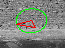
\includegraphics[width=\linewidth]{FIGS/TaskCorrel/EllipseAffine/ElspA.png}
        \end{subfigure}%
        	\hfill
        \begin{subfigure}[b]{0.16\textwidth}
                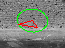
\includegraphics[width=\linewidth]{FIGS/TaskCorrel/EllipseAffine/ElspB.png}
        \end{subfigure}%
                \hfill
        \begin{subfigure}[b]{0.16\textwidth}
                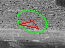
\includegraphics[width=\linewidth]{FIGS/TaskCorrel/EllipseAffine/ElspC.png}
        \end{subfigure}%
                \hfill
        \begin{subfigure}[b]{0.16\textwidth}
                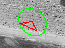
\includegraphics[width=\linewidth]{FIGS/TaskCorrel/EllipseAffine/ElspD.png}
        \end{subfigure}
                \hfill
        \begin{subfigure}[b]{0.16\textwidth}
                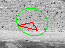
\includegraphics[width=\linewidth]{FIGS/TaskCorrel/EllipseAffine/ElspE.png}
        \end{subfigure}
                 \hfill
        \begin{subfigure}[b]{0.16\textwidth}
                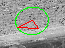
\includegraphics[width=\linewidth]{FIGS/TaskCorrel/EllipseAffine/ElspF.png}
        \end{subfigure}
        \newline
        \begin{subfigure}[b]{0.16\textwidth}
                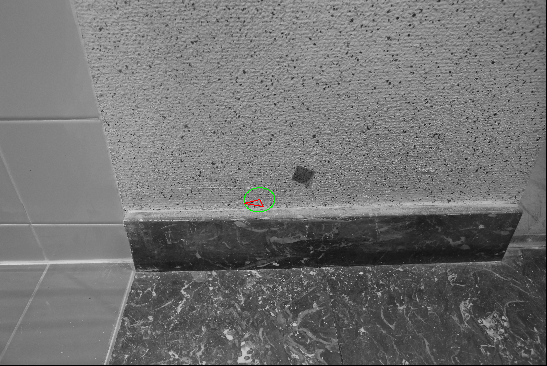
\includegraphics[width=\linewidth]{FIGS/TaskCorrel/EllipseAffine/imgA.png}
        \end{subfigure}%
        	\hfill
        \begin{subfigure}[b]{0.16\textwidth}
                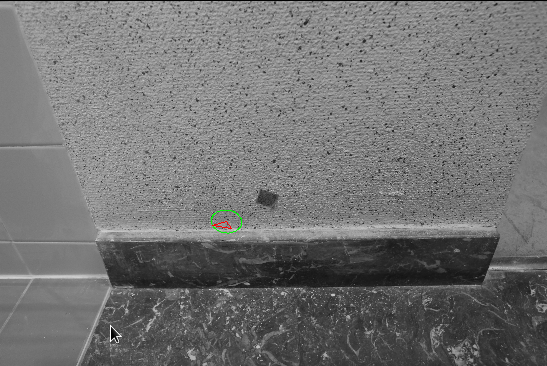
\includegraphics[width=\linewidth]{FIGS/TaskCorrel/EllipseAffine/imgB.png}
        \end{subfigure}%
                \hfill
        \begin{subfigure}[b]{0.16\textwidth}
                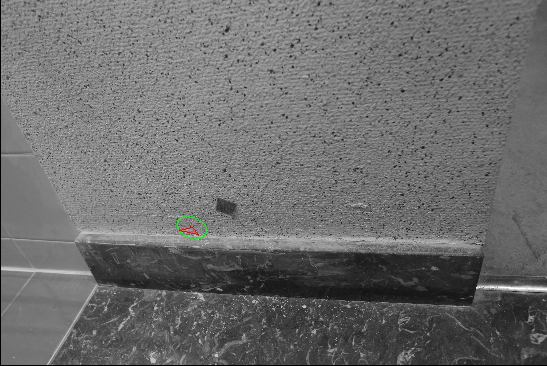
\includegraphics[width=\linewidth]{FIGS/TaskCorrel/EllipseAffine/imgC.png}
        \end{subfigure}%
                \hfill
        \begin{subfigure}[b]{0.16\textwidth}
                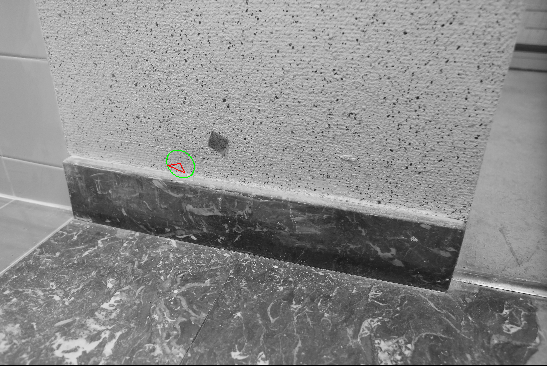
\includegraphics[width=\linewidth]{FIGS/TaskCorrel/EllipseAffine/imgD.png}
        \end{subfigure}
                \hfill
        \begin{subfigure}[b]{0.16\textwidth}
                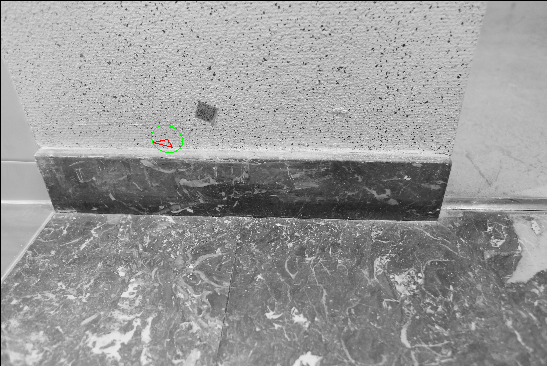
\includegraphics[width=\linewidth]{FIGS/TaskCorrel/EllipseAffine/imgE.png}
        \end{subfigure}
                 \hfill
        \begin{subfigure}[b]{0.16\textwidth}
                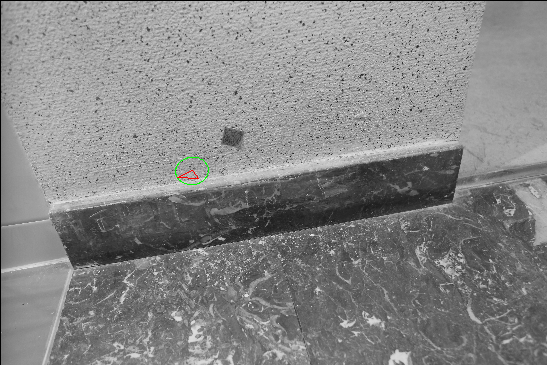
\includegraphics[width=\linewidth]{FIGS/TaskCorrel/EllipseAffine/imgF.png}
        \end{subfigure}
        \caption{Condition of optimal resolution based on deformation of ellipse through different visual direction. In this case, the most right image will be choosen as image master for the 3D triangle considered}
        \label{fig:ellipse_deform}
\end{figure}

\item Detection interest points:
\begin{itemize}
\item Create affine invariant regions (interest region) for each image of each image pair master–slave in group.
These regions are given by the projection of triangle 3D on each image. 
Interest region in image slave will be transformed to image master geometry by an affine estimated from correspondent coordinates of triangle projected ‘s peaks.
\item A detection of interest points is performed on these regions. This detection using multi conditions to select point interest suitable for matching by correlation. The risk of repetitive patterns and low contrast that could cause fail matching by correlation is also handle.
\end{itemize}

\item Optimal correlation for matching:
\begin{itemize}
\item For each interest point in interest region of image master, points candidate for matching are chosen in image slave.
\item The optimal correlation matches each pair of interest points on multi scale to ameliorate speed and accuracy.
\item Correlation search for best match in three scale level. An independent threshold applied at each level to quickly eliminate non potential match pair. 
\begin{itemize}
 \item A quick correlation with 2 pixel scale without interpolation (consider 1 pixel every 2 pixels).
 \item An original scale correlation (entier of pixel - original image resolution). 
 \item A sub-pixel correaltion at 0.01 pixel (by interpolation image original). 
\end{itemize}
\end{itemize}
After matching procedure, a spatial filter is applied to keep a uniform distribution of tie points on image. 

\end{enumerate}




\subsection{New tie-point extraction procedure}
\subsubsection{Input data requirements}
\begin{itemize}
  \item A mesh triangulation (can be generated from point cloud by {\tt TiPunch}) 
  \item Images orientations (Ori-XXX folder computed by {\tt Tapas} for example)
  \item Cameras calibrations (Ori-XXX/AutoCalXXX - computed by {\tt Tapas} for example)
\end{itemize}
\subsubsection{First step: Selection images by {\tt TestLib TaskCorrel}}
\begin{verbatim}
mm3d TestLib TaskCorrel


********************************************************
*    TaskCorrel - creat XML for TiepTri                *
********************************************************
*****************************
*  Help for Elise Arg main  *
*****************************
Mandatory unnamed args : 
  * string :: {Pattern of images}
  * string :: {Input Initial Orientation}
  * string :: {path to mesh(.ply) file - created by Inital Ori}
Named args : 
  * [Name=xmlCpl] string :: {file contain couple of image - processe by couple}
  * [Name=assum1er] bool :: {always use 1er pose as img master, default=0}
  * [Name=useExist] bool :: {use exist homol struct - default = false}
  * [Name=angleV] REAL :: {limit view angle - default = 90 (all triangle is viewable)}
  * [Name=OutXML] string :: {Output directory for XML File. Default = XML_TiepTri}
  * [Name=Test] bool :: {Test stretching}
  * [Name=nInt] INT :: {nInteraction}
  * [Name=aZ] REAL :: {aZoom image display}
  * [Name=aZEl] REAL :: {fix size ellipse display (in pxl)}
  * [Name=clIni] Pt3dr :: {color mesh (=[255,255,255])}
  * [Name=distMax] REAL :: {Limit distant process from camera}
  * [Name=rech] INT :: {calcul ZBuffer in Reechantilonage (def=2)}

\end{verbatim}

The meaning of main parameters is:

\begin{itemize}
   \item mandatory parameter: the pattern of images.
   
   \item mandatory parameter: orientation relative.
   
   \item mandatory parameter: mesh file (in coordonate relative coherent with orientation relative above).

   \item  {\tt OutXML} Suffix for output folder (will contain XML file for the next command)

   \item  {\tt distMax} Distant maximum to consider from image (use to calculate ZBuffer and to limit in case of large scenario) 

   \item  {\tt rech} DeZoom for calculate ZBuffer (def=2 => 1/2 resolution image);

\end{itemize}


Output of the command is XML files for each images.


\subsubsection{Second step: Extraction tie-point with {\tt TiepTri}}

\subsubsection{Third step: Compensation images orientations and calibration with  {\tt Campari}}

\subsection{An example}

%=======================================================================================================

